\documentclass[english]{article}
\usepackage[latin9]{inputenc}
\usepackage[letterpaper]{geometry}
\usepackage{textcomp}
\usepackage{soul}
\usepackage{tabularx}
\usepackage{booktabs}
\usepackage{graphicx}
\usepackage{xparse}
\usepackage{hhline}
\setlength{\heavyrulewidth}{1pt}
\setlength{\abovetopsep}{2pt}
\usepackage{float}
\restylefloat{table}
\geometry{verbose,tmargin=1in,bmargin=1in,lmargin=1in,rmargin=1in}

\begin{document}

%*********** Use this for project proposal ************
% \emph{\footnotesize{CIS 520 Fall 2019, Project Proposal}}

%*********** Use this for project checkpoint ************
% \emph{\footnotesize{CIS 520 Fall 2019, Project Checkpoint}}

%*********** Use this for project report ************
\emph{\footnotesize{CIS 520 Fall 2019, Project Report}}

\vspace{12pt}


%*********** Use this header for project checkpoint, feel free to modify for final report ************

%Fill in your project title
\textbf{\Large{YouTube Video Popularity Prediction Using View Counts as Criteria with Classification Models and Neural Networks}}

\vspace{1cm}

\textbf{Team Members:}

%Fill in your team details; remove any lines that are not needed
\begin{itemize}
 \item Hanxiang Pan; Email: \texttt{henrypan@seas.upenn.edu}
 \item Jialin Lou; Email: \texttt{joyljl@seas.upenn.edu}
 \item Zijie Song; Email: \texttt{szjjay74@seas.upenn.edu} 
\end{itemize}

\hline

%*********** Use this to include abstract in project report (comment out in project proposal) ************

\begin{abstract}
Video popularity prediction is of great importance in nowadays social media world. How did some videos go virus while others not? How did YouTube decide videos in "Trending now" section? These are all questions video popularity prediction tries to solve. The goal of this report is to use machine learning to predict the popularity of YouTube videos. We present 2 models using machine learning based on regarding "view counts" as popularity criterion. \\\\
\textbf{Keywords:} Sentimental Analysis, Text classification, Dimension Reduction, Text Frequency Inverse Document Frequency (TF-IDF), Convolutional Neural Network
\end{abstract}


%*********** Recommended section structure for project report and checkpoint below (comment out in project proposal) ************

\section{Motivation}

With the ever lowering entry barrier for video publication on platforms like YouTube and Instagram, more and more people start to consider these platforms as simple way to convey their ideas and these platforms start to play a more significant role in people's life. These platforms has also developed a trend for people to know others around the world as well as for the world to know you. With more sponsors pouring more money on creators, predicting the popularity of a new upcoming video upload has its business importance. We want to create a model to predict how popular a video might become to assist with such business decisions.

\section{Related Work}
%\textit{Tip: we suggest using bibtex for easy citation management. For example, here are citations to Bishop's book \cite{Bishop06} and the UCI machine learning repository \cite{DuaKa17}.} \\ \\
To come up with our unique solution to the proposed problem, we referenced these two publications. 
\begin{itemize}
    \item The first publication named \textit{Web Video Popularity Prediction using Sentiment and Content Visual Features} \cite{vp1} showcased a way to integrate sentiment features on titles and content visual features (thumbnails) into popularity analysis.
    \item The second publication we found named \textit{Popularity Prediction of Videos in YouTube as Case Study: A Regression Analysis Study} \cite{vp2} showcased logistic regression for predicting popularity based on a variety number of features, and used step-wise regression to pick out a minimum number of features to maximize prediction accuracy.
\end{itemize}

\section{Data Set}
Datasets:
\begin{itemize}
\item Trending Youtube Video Stats: https://www.kaggle.com/datasnaek/youtube-new
\item Youtube Channels: https://www.kaggle.com/babikov/youtube-channels-100000
\item Trending Youtube (with comments): https://www.kaggle.com/datasnaek/youtube
\end{itemize}
\item $\textbf{N}$ - number of youtube trending videos
\item $\textbf{p}$ - related features: trending date, title, channel title, category, publish time, tags, views, likes, dislike, comment count, thumbnail, video description, is comments disabled, is rating disabled, comments


\section{Problem Formulation}
\begin{enumerate}
    Our task is to predict popularity of a specified YouTube video. To convert this task into machine learning task, we chose the "view counts" as a criterion of popularity and use the features such as categories, descriptions, titles, and tags of videos, to classify the level of popularity. Since for popular videos, the numbers of view counts are often really big, to make our prediction more meaningful, we will split our "view counts" into buckets with specified range. These 10 buckets will represent 10 different levels of popularity. Then we will use these labels as our classification target.\\ \\
    \subsection{How did we choose $y$?}
    % \begin{enumerate}
    %     \item We chose "view counts" as a proxy for determining the popularity of a video.
    %     \item Create 10 levels of popularity specified in the chart below based on range of "view counts", with equal number of samples in each bucket [\ref{Bucket Redesign}].\\ \\
    %     \begin{tabular}{||c||c||c||}
    %     \hhline{|=|=|=|}
    %     \textbf{Level of Popularity}&\textbf{Min of bucket view counts}&\textbf{Max of bucket view counts}\\
    %     \hhline{|=|=|=|}
    %         1 &548  &95485\\
    %         2 &95486  &211792\\
    %         3 &211793  &332001\\
    %         4 &332002  &495256\\
    %         5 &495257  &718073\\
    %         6 &718074  &1029140\\
    %         7 &1029141  &1485263\\
    %         8 &1485264  &2326589\\
    %         9 &2326590  &4492755\\
    %         10 &4492756  &225211924\\
    %     \hhline{|=|=|=|}
    %     \end{tabular}\\
    %     \item $y \in Y = \{0,1,2,3,4,5,6,7,8,9\}$
    % \end{enumerate}

    \subsection{What features did we use?}
    % \begin{enumerate}
    % \begin{tabular}{||c||c||c||}
    %     \hhline{|=|=|=|}
    %     \textbf{Feature}&\textbf{Description}&\textbf{Usage}\\
    %     \hhline{|=|=|=|}
    %      Description & Text content in "description" & Converted into embedding space, see note\\
    %      Tags & Text content in "tags" & Converted into embedding space, see note\\
    %      Titles & Text content in "title" & Converted into embedding space, see note\\
    %      Click-bait &  Click-bait score evolves from content in "title" & Click-bait score from 0-1\\
    %      Category & Category index from 1-43 & One-hot encoding for existing category\\
    %     \hhline{|=|=|=|}
    %     \end{tabular}\\ \\
    %      Note: The word vector - Global Vectors for Word Representation (GloVe) \cite{pennington2014glove} that we used for converting raw text into embedding features is pre-trained on Twitter data, containing 2 billion tweets, 27 billion tokens and 1.2 million vocabulary.

    % \end{enumerate}
    
\end{enumerate}



\section{Methods}
\begin{enumerate}
    
    \subsection{Pre-processing}
    \label{preprocess}
    \begin{enumerate}
    \item Filter out videos that don't allow comments and ratings or videos that are removed.
    \item Add a new feature named ``trending\_period" calculated as ``publish\_date - trending\_date".
    \item Add a new feature named ``invalid\_thumbnail" to filter out data whose thumbnails are not available.
    \item Remove non-ascii characters, stopwords, punctuactions and tokens with leading punctuations in the ``description", ``title", ``channel\_title", and ``tags".
    \item Split content in ``description", ``title", ``channel\_title", and ``tags" into tokens.
    \item Draw category id distribution and trending period distribution.
    \item Draw title's word cloud over each categories.\\
    % \begin{figure}[!htb]
    % \minipage{0.32\textwidth}
    %   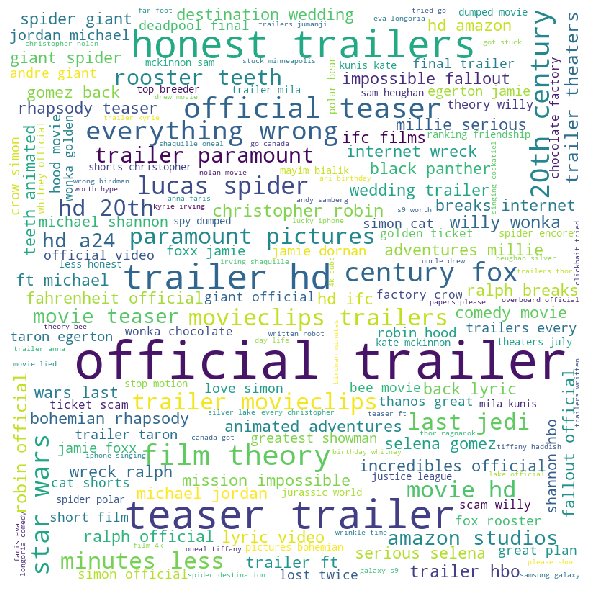
\includegraphics[width=\linewidth]{project/wc_1.png}
    %   \caption{Film \& Animation}\label{fig:awesome_image1}
    % \endminipage\hfill
    % \minipage{0.32\textwidth}
    %   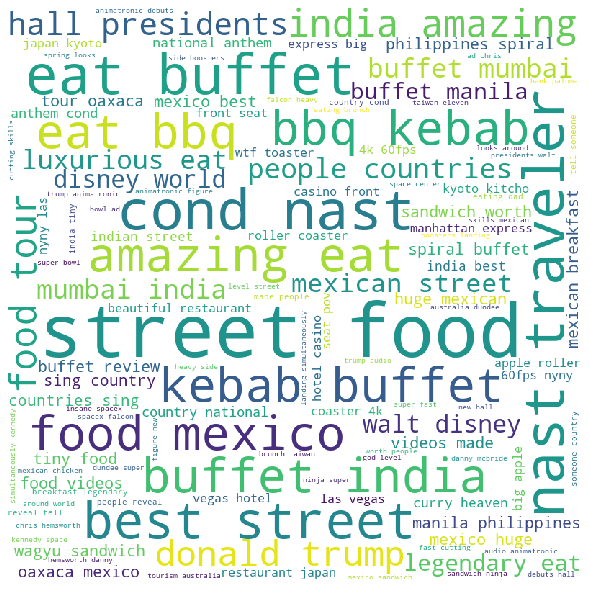
\includegraphics[width=\linewidth]{project/wc_19.png}
    %   \caption{Travel \& Events}\label{fig:awesome_image2}
    % \endminipage\hfill
    % \minipage{0.32\textwidth}%
    %   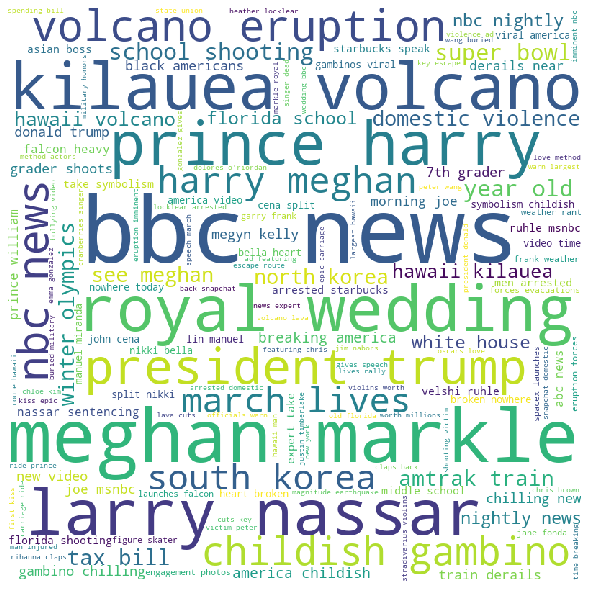
\includegraphics[width=\linewidth]{project/wc_25.png}
    %   \caption{News \& Politics} \label{fig:awesome_image3}
    % \endminipage
    % \end{figure}

    \end{enumerate}
    
    \subsection{Feature extraction}
    \begin{itemize}
    \item Generate a word bank through removing top 10\% most frequent cleaned tags for each category in the data to avoid over-weighting the word bank. The format of the word bank: 
    \{category\_id: list of cleaned tags\}.
    \item Use tokens generated 5.1.(e) step in description to generate potential category(ies) based on its frequency in the word bank. In addition to the single category provided in the original dataset, we have augmented the data with a total of 16 categories across all our samples. This provides more features for our classification problem.
    \item Use CountVectorizer to convert a text documents to a matrix of token counts.
    \item Use TF-IDF with PCA to train and transform training data.
    \item Use GloVe embeddings to extract our feature's corresponding embedding index from the trained corpus. This is used as the initial weights for the embedding neural network layer. 
    \item Convert the category index into one-hot encoding and encode them with TF-IDF features (developed in step 5.2.(d)) / GloVe embeddings (developed in step 5.2.(e)).
    \end{itemize}
    
    \subsection{Classification/Prediction}
    \begin{itemize}
        \item Multi-layer perceptron model for classification
        \item Multi-layer Convolutional Neural Network for classification
    \end{itemize}
    
    \subsection{Baseline Discussion}
    We used the pre-processed dataset from \ref{preprocess} and only used TF-IDF features with respect to each of the three fields ($title$, $description$, $tags$) for the baseline. The hyper-parameters were default values provided by the scikit-learn library. We wanted to see whether the problem formulation and the $y$ target value definition was reasonable. The experiment and results can be found in \ref{Bucket Redesign}.

\end{enumerate}

\section{Experiments and Results}
\subsection{Experiment 1}
\subsubsection{Experiment}
\begin{enumerate}
\item Instead of predicting specific view counts, this problem can be converted into classifying videos into view count buckets, where each bucket contains a view count range (e.g. 1 million to 2 million views). We split the view count, based on the min/max range of all the view counts, into 10 uniform buckets, while keeping interval size of each bucket the same. 
\item Convert ``views" for each sample in the dataset into a one-hot categorical label, corresponding to a bucket/class.
\item Construct and transformed raw text data into TF-IDF training/testing data, one feature at a time For this experiment, we used ``tag", ``description and ``title". 
\item Train a naive bayes model on transformed TF-IDF data and the labels generated from step (b).
\item Run the classifier to classify the test data into specific view buckets
\end{enumerate}
\subsubsection{Results}
\begin{itemize}
    \item The results show that the most of classifications were concentrated in the first bucket, which led to further investigation of our bucket design and our second experiment.
    \item The investigation show that our input data had a right-skewed distribution for the ``views" feature, which led to the first two buckets to cover 90\% of all the samples.
    % \begin{figure}[H]
    %     \centering
    %     \resizebox{4in}{!}{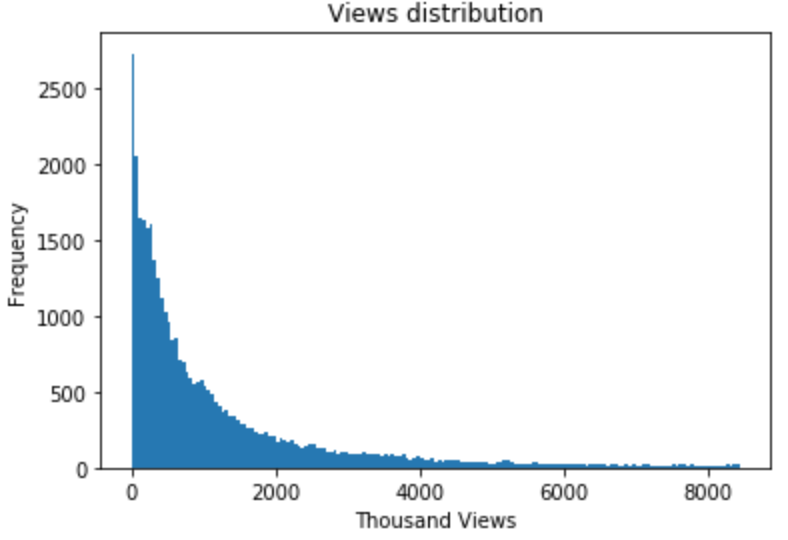
\includegraphics{project/view_distribution.png}}
    %     \caption{Views Distribution}
    %     \label{fig:my_label}
    % \end{figure}
    
\end{itemize}

\subsection{Experiment 2 (Baseline)}
\subsubsection{Experiment}
\label{Bucket Redesign}
\begin{enumerate}
\item Split the raw view count, based on view count percentiles, into 10 uniform buckets, which keeps number of samples in each bucket the same. 
\item Convert ``views" for each sample in the dataset into a one-hot categorical label, corresponding to a bucket/class.
\item Train the same Naive Bayes classifier (in experiment 1), to verify that the bucket design alleviates the problem of having a skewed data distribution. For this experiment, we also only used ``tag", ``description" and ``title", one feature at a time.
\item Train the data on various of classifiers such as the random forest classifier, ridge regression classifier, stochastic gradient descent classifier, boosted gradient trees, and linear-SVM (one-vs-rest and one-vs-one scheme).
\item Run the classifier to classify test data into specific view buckets. We used ``title",``tags", and ``description" respectively to predict the view buckets on the test data.
\end{enumerate}

\subsubsection{Results}
\begin{itemize}
\item The resulting redesign of the view buckets has a distribution of a uniform across all buckets (rectangular shape).
\item{Classification Accuracy Comparison}
% \begin{table}[H]
%     \centering
%     \begin{tabular}{ *2c } 
%      \toprule
%      \textbf{Method} & \textbf{Accuracy (\%)}\\
%      \midrule
%      \multicolumn{2}{c}{\textit{Tags}} \\
%      \midrule
%      Ridge & 50.6 \\
%      Linear SVM (one-vs-rest) & 49.2 \\
%      Naive Bayes & 47.2 \\
%      SGD & 44.5 \\
%      Random Forest & 29.5 \\
%      Gradient Tree Boosting & 26.5 \\
%      Linear SVM (one-vs-one) & 14.1 \\
%      \midrule
%      \multicolumn{2}{c}{\textit{Description}} \\
%      \midrule
%      Naive Bayes & 33.0 \\
%      Ridge & 27.9 \\
%      SGD & 26.6 \\
%      Linear SVM (one-vs-rest) & 26.3 \\
%      Gradient Tree Boosting & 16.6 \\
%      Random Forest & 13.5 \\
%      Linear SVM (one-vs-one) & 12.2 \\
%      \midrule
%      \multicolumn{2}{c}{\textit{Title}} \\
%      \midrule
%      Naive Bayes & 21.8 \\
%      Ridge & 20.8 \\
%      Linear SVM (one-vs-rest) & 20.2 \\
%      SGD & 20.2 \\
%      Linear SVM (one-vs-one) & 17.2 \\
%      Gradient Tree Boosting & 13.9 \\
%      Random Forest & 13.6 \\
%      \bottomrule
%     \end{tabular}
%     \label{nnOA}
%     \end{table}

\end{itemize}

%\pagebreak
\subsection{Experiment 3}
\subsubsection{Experiment}
\begin{enumerate}
\item Use PCA on TF-IDF transformed data generated in 6.1.1.(3) (TF-IDF matrix with text content in "tags","description", and "title" field) and draw the components vs. variance explained graph to select number of components.
% \begin{figure}[H]
%     \centering
%     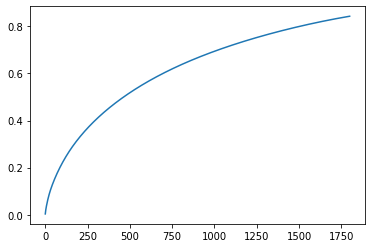
\includegraphics[width=0.5\textwidth]{project/pca.png}
%     \caption{Number of components vs. Variance explained}
%     \label{fig:pca}
% \end{figure}
We found that when the number of components is 1800, we can get over 80\% of variance explained. Therefore, we choose 1800 components after applying PCA on TF-IDF transformed matrix.
\item Since popularity is tightly related to category, videos in different categories have different minimum and maximum view counts. Therefore, we are going to encode video category into our feature matrix. We will use one-hot encoding for 16 categories that appeared in our data in order to avoid giving extra weight to videos who belong to a category which index number is large.
\item We found an open-source of a click-bait score detector\cite{click-bait}, we used this detector to generate a click-bait score that ranging from 0-1 as a new feature to predict video popularity.
\item Combined TF-IDF matrix with click-bait score and category one-hot encoding. Our final feature matrix for experiment 3 looks like: \\
    TF-IDF matrix after PCA  + Click-bait score  + one-hot encoding category\\
    (1800 columns) + (1 columns)  +  (16 columns)
\end{enumerate}
\subsubsection{Results}
%     \begin{itemize}
%     \item Train a Multi-Layer Perceptron (MLP) classifier on the features we generated from step 4) with max\_iter = 500 (Stopped at 363rd iteration). \\
%     \begin{figure}[H]
%     \centering
%     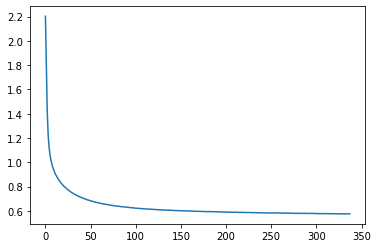
\includegraphics[width=0.5\textwidth]{project/mlp.png}
%     \caption{Number of iterations vs. loss}
%     \label{fig:mlp}
% \end{figure} 
% The MLP classifier achieve a test accuracy of 67.8953\% and a training accuracy of 76.9646\%.
% \end{itemize}

\subsection{Experiment 4}
\subsubsection{Experiment}
\begin{enumerate}
\item Considering that different channels would also affect the popularity of videos, we would like to incorporate YouTube Channels dataset with our Trending YouTube Video Stats dataset.
\item Merge 2 datasets together on $channel\_title$ and include the following features:
\begin{itemize}
    \item category one-hot encoding
    \item TF-IDF
    \item number of channel subscribers (new feature)
    \item number of videos posted by channels (new feature)
\end{itemize}
\item Our final feature matrix for experiment 4 looks like: \\
    TF-IDF matrix after PCA  + Click-bait score  + one-hot encoding category + number of channel subscribers + number of videos posted by channels \\
    (1800 columns) + (1 columns)  +  (16 columns) + (1 columns) + (1 columns) 
\end{enumerate}
\subsubsection{Results}
    \begin{itemize}
    \item Train a MLP classifier on the features we generated from step 4) with max\_iter = 500 (Stopped at 338th iteration).
    \item The MLP classifier achieve a test accuracy of 9.5648\%, which is extremely low. We did further examine of our dataset and found out that the view counts of the videos do not seem to relate to the number of channel subscribers and number of videos of a channel. Therefore, we decided not to add these new features.
\end{itemize}


\subsection{Experiment 5}
\subsubsection{Experiment}
\begin{enumerate}
    \item Loaded the pre-trained word vector GloVe
    \item Used GloVe embeddings as the basis for extracting our feature's corresponding embedding index in the trained corpus. This is used as the initial weights for the embedding neural network layer. 
    \item Similar to our previous experiments, we converted $views$ into discrete bucket ranges with a total of 10 buckets, with each bucket containing the same number of samples
    \item Loaded preprocessed feature data, including title, description and tags
    \item Encoded each feature document into an integer which indicates its sequence index
    \item Padded all feature documents to the same length to unify data shape for model training
    \item Created a weight matrix containing the embeddings for each of the feature 
    \item Split data into 75\% training and 25\% testing set
    \item Converted the buckets into one-hot encoding instead of 0-9 integers
    \item Concatenated the one-hot categories for each sample to the output of the global max pooling layer and feed into the next fully-connected layer "dense\_56"
    \item Trained and evaluated the model on a multi-layer neural network, optimized using a categorical cross-entropy loss function
    
    \noindent \textbf{Neural Network Architecture}
    
    % \begin{figure}[H]
    %   \centering
    %     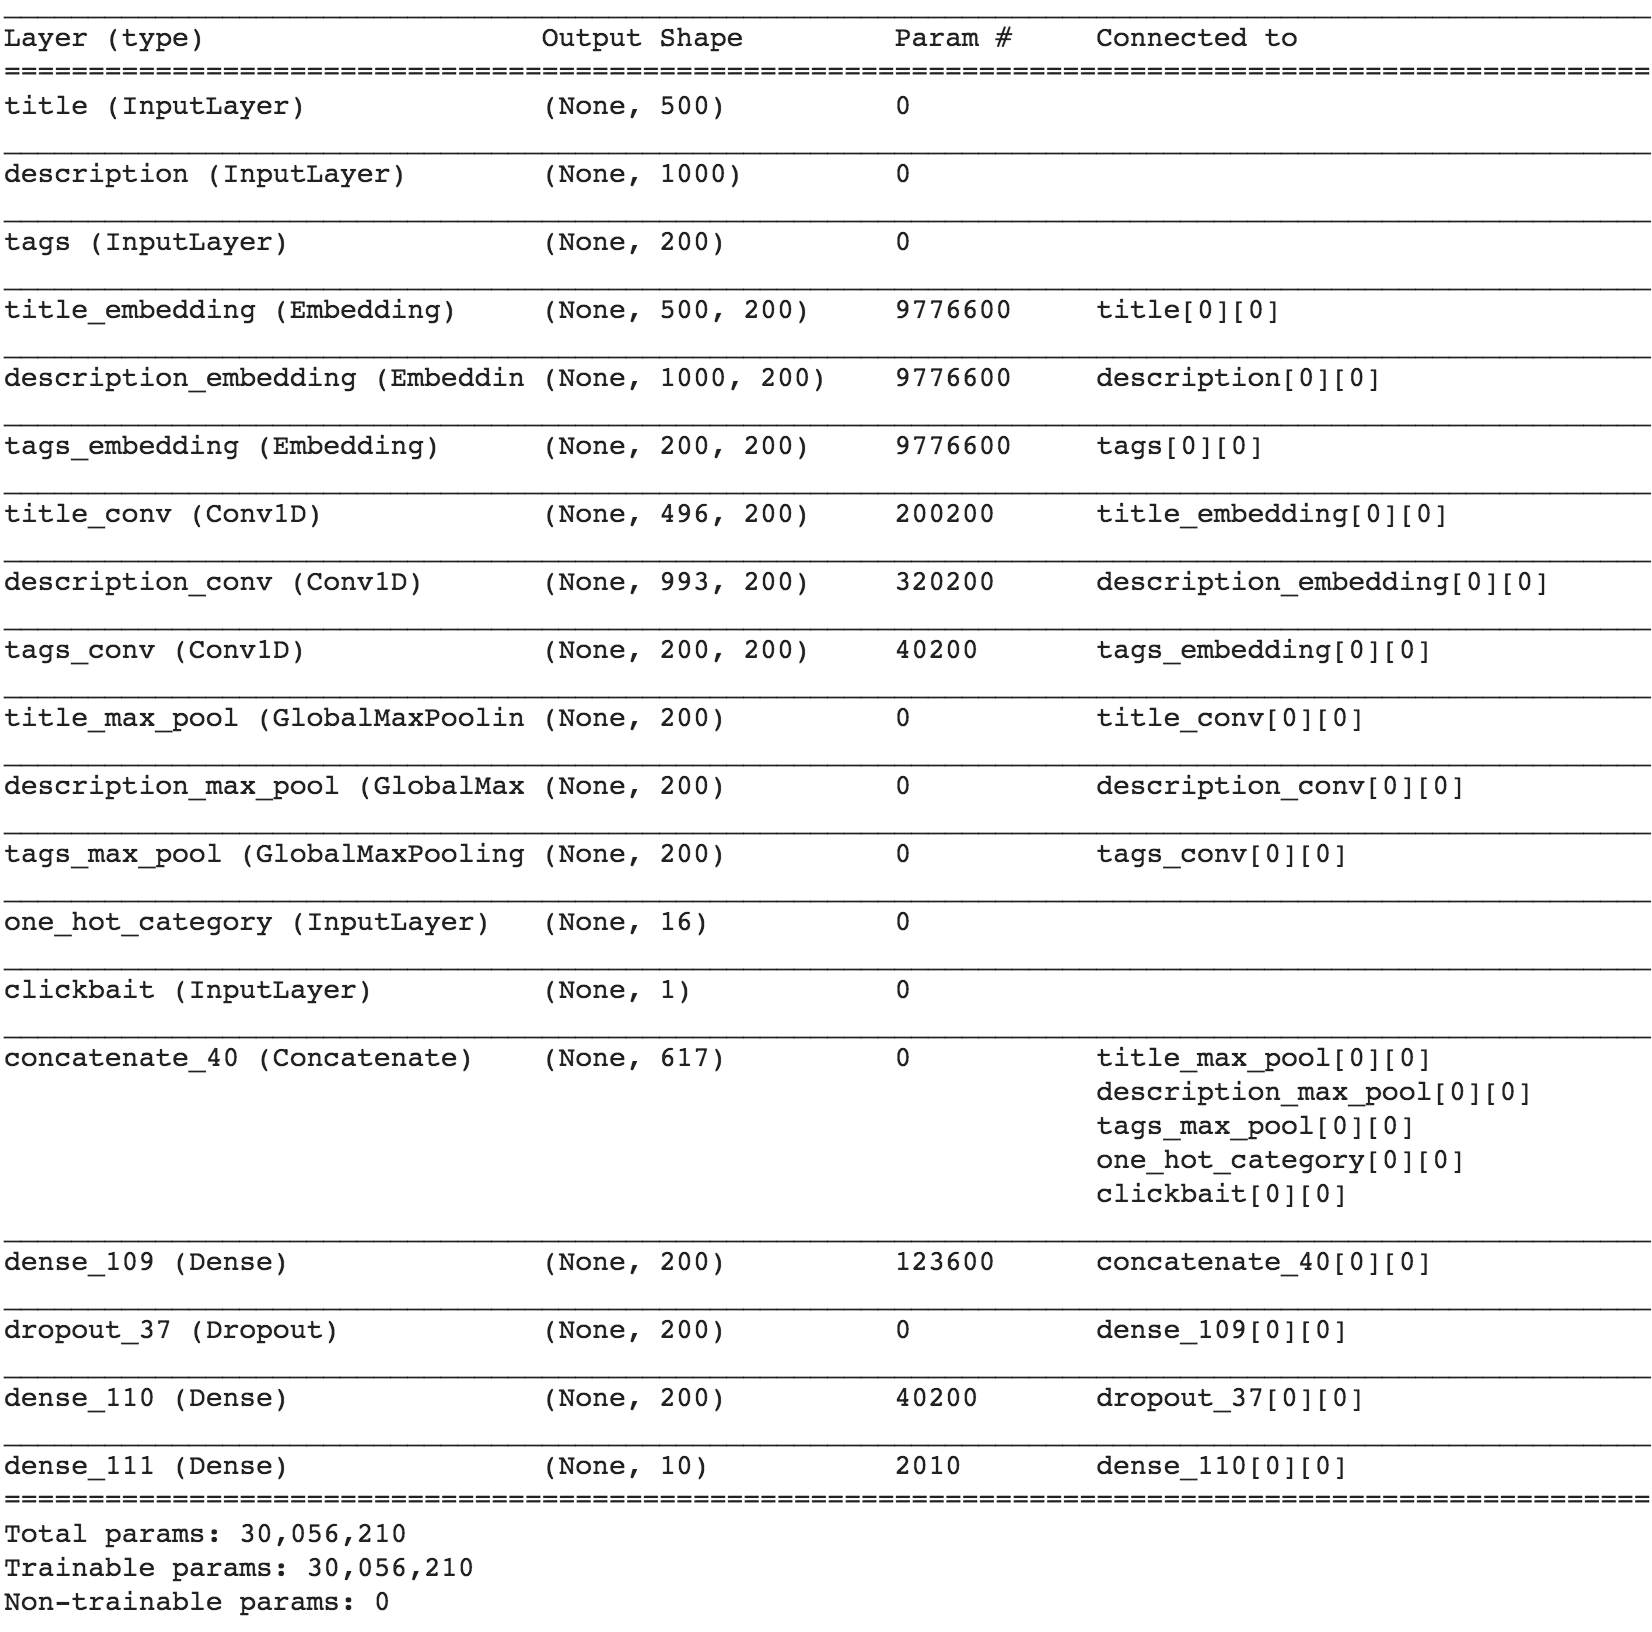
\includegraphics[scale=0.5]{nn_1.png}
    %     \caption{Twitter 200d Embedding}
    % \end{figure}
    
    The reason for the above neural network architecture is as follows:
    \begin{itemize}
        \item We want to have a good starting point for our weights, which we've used the gloVE as our initial embedding layer weights. Then, we attempted to transfer learn "Twitter" domain embeddings to "Youtube" domain embeddings.
        \item For text, there are some contextual information embedded in the sequence of words. The $Conv1D$ layer is used to extract useful features from a small patch of that embedded sequence.
        \item To prepare our features for concatenation with our non-textual features (category one-hot encoding), we apply the max pooling layer after the convolution layer.
        \item After concatenating the category features with the main set of features from the max pooling layer, we apply two more fully-connected layers to learn more high level features.
        \item To reduce overfitting, we added a drop-out layer with 20\% drop-out rate, in between the last and second-last fully-connected layer.
        \item Finally, we used a non-linear $sigmoid$ activation function at last layer to "squeeze" the dimensions down to 10 for our 10-class classification problem.
    \end{itemize}

\end{enumerate}
\subsubsection{Hyper-Parameters}
\begin{itemize}
    \item Maximum length document: 1000 (Description)
    \item Maximum length document: 500 (Title)
    \item Maximum length document: 200 (Tags)
    \item Conv1D number of filters: 200 (Defined by pre-trained embedding dimension)\\
    kernel size: 8 (description)\\
    kernel size: 5 (title)\\
    kernel size: 1 (tags)\\
    stride size: 1 (title, tags, description)
    \item Learning rate: 0.001
\end{itemize}

\subsubsection{Results}
\begin{itemize}
    \item We decided to make the embedding layer weights trainable (since the pre-trained embedding is not the same domain as our problem, it might make sense to use the weights as a starting point and train it ourselves.
    \item Training Loss and Accuracy
    % \begin{figure}[H]
    %   \centering
    %     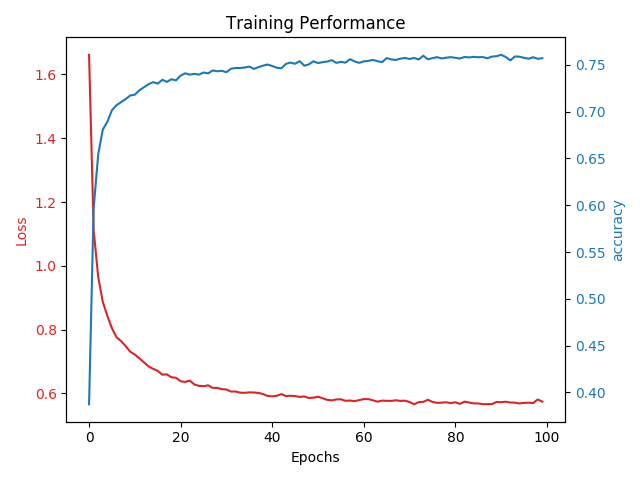
\includegraphics[scale=0.5]{loss_1.png}
    %     \caption{Title, Description, Tags $|$ Twitter 200d Embedding $|$ CNN $|$ (Test Accuracy 68.5\%))}
    % \end{figure}
    
    % The training loss converges to 0.6, and the training accuracy converges to 75\% after after around 25 episodes.
    
    % \begin{figure}[H]
    %   \centering
    %     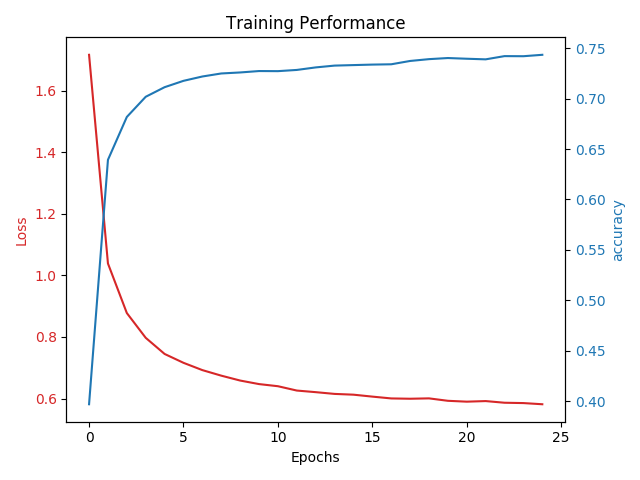
\includegraphics[scale=0.5]{loss_2.png}
    %     \caption{Title $|$ Twitter 200d Embedding $|$ CNN $|$ (Test Accuracy 67.72\%))}
    % \end{figure}
    
    The training loss converges to 0.6, and the training accuracy converges to 74\% after after around 25 episodes.
    
    \item Test Accuracy
    % \begin{table}[H]
    % \centering
    % \begin{tabular}{ *2c } 
    %  \toprule
    %  \textbf{Features} & \textbf{Test Accuracy (\%)}\\
    %  \midrule
    %  Title, Description, Tags, Category & 68.5 \\
    %  Title, Category & 67.72 \\
    %  \bottomrule
    % \end{tabular}
    % \label{nnOA}
    % \end{table}
    
    It seems that by including more features, it does improve the test accuracy slightly. As a future step, these text-based features might need separate neural networks for extracting features, as their contexts are different.


\end{itemize}



\section{Conclusion and Discussion}

After experimenting with various feature extraction methods and classification approaches, the combination that yielded the best performance is as follows:

\begin{itemize}
    \item Data pre-processing is done by tokenizing the text fields $title$, $description$, and $tags$, and removing stopwords and irrelevant symbols.
    \item In addition to the single category feature that is part of each video. It is helpful to augment additional category features since we noticed that some videos were cross-disciplinary videos (comedy show about politics should attribute to at least two categories, entertainment and politics).
    \item Adding a "clickbait" feature based on the "title" of every video
    \item Our objective is to classify each video into a bucket that represents a range of view counts, but also ensuring that when we defined the buckets, each bucket contained the same number of samples.
    \item The results of fine-tuning a pre-trained Twitter language embedding model using CNN was similar to using a multi-layered perceptron network. However, the CNN model was more complex which might have led to underfitting. 
    
\end{itemize}

\textbf{Insights:} This problem is an interesting one. Despite that we don't know how "trending" YouTube videos gain its viewership, and not considering any video or image data as part of the scope of this project, we still managed to reach an approximate 68\% test accuracy rate (significantly better than 10\% guessing) for predicting whether a video will become popular. We intentionally left out $like/dislike\ counts$, $comment\ counts$ from our model, because our problem definition is to predict whether a new video upload will become popular. Those data are generated after a video is viewed, so we didn't want to mix up the causal relationship when dealing with prediction problems.\\

\textbf{Lessons:} When performing any kind of feature transformation such as converting a view count into a set of discrete view count buckets, it is imperative to check the distribution of the output data since the input data might be very skewed, which results in a very biased discretization. This would ultimately give too much weight on a particular set of samples. \\

\textbf{Future Steps:} 
\begin{itemize}
    \item Our dataset is limited to "trending" videos. These videos have been picked out by YouTube's algorithms, and therefore, doesn't represent a fresh new upload. As an extension, we could try to use a dataset that contains normal videos and their associated metadata. 
    \item In addition to text features, we could try to incorporate thumbnail image features. Intuitively, we believe that users are somewhat swayed by the first impression of the thumbnail. "Clickbait" analysis can also be applied to these image features.
    \item From a neural network architecture perspective, we could try other methods of combining the embedding features with other numerical features (e.g. video category). The current approach of concatenating them might lead to numerical biases.
\end{itemize}


%\section*{Acknowledgments}

\newpage
%============================= BIBLIOGRAPHY ===============================

\bibliographystyle{plain}
\bibliography{references}

\end{document}